\chapter{Phase de développement~: conception et implémentation d'un module
statistique}
	\paragraph{}
	Dans la partie précédente nous avons proposé une solution fonctionnelle aux
	besoins exprimés par les utilisateurs. Ici, nous allons concevoir une solution
	technique à partir des focntionnalités, puis l'implémenter. La partie A
	présentera l'architecture actuelle de TrackCIS, dans la partie B nous
	conceverons la solution technique et la partie C présentera la méthodologie
	d'implémentation de cette solution. Enfin, dans la partie D, nous ferons le
	bilan de ce qui a effectivement pus être implémenté au cours de ce projet et
	nous discuterons des limites et des biais de la méthodologie ainsi que des
	suites possibles pour Xperis.
	
	\section{TrackCIS, une application web en deux parties}
		
		\subsection{Qu'est-ce qu'une application web ?}
			\paragraph{}% Modèle client serveur classique
			TrackCIS est une application accessible depuis un navigateur internet, il
			s'agit d'une application web. Le fonctionnement de cet type d'application est
			basé sur le modèle client-serveur. Un client correspond au navigateur
			internet de l'utilisateur (Chrome, FireFox\ldots), il permet de communiquer
			avec le serveur. Le serveur est la machine sur
			laquelle est déployée l'application web. Le client envoie une requête au
			serveur qui va la traiter et produire en retour une page web, c'est-à-dire
			une page HTML (Hypertext Markup Language) laquelle va être renvoyée au client
			et affichée.
			
			Il est installé au niveau d'un serveur,
			généralement citué au sein de l'établissement hospitalier et connecté au
			réseau local. La machine de l'utilisateur, que l'on appel le client, ce
			connecte à ce serveur. Ce dernier reçoit de la part du client une requête
			HTTP (protocole standard d'échange sur internet).
			% Le client fait une requête à laquelle le serveur répond en envoyant une
			% page HTML
			
			\begin{figure}[H]
				\centering
				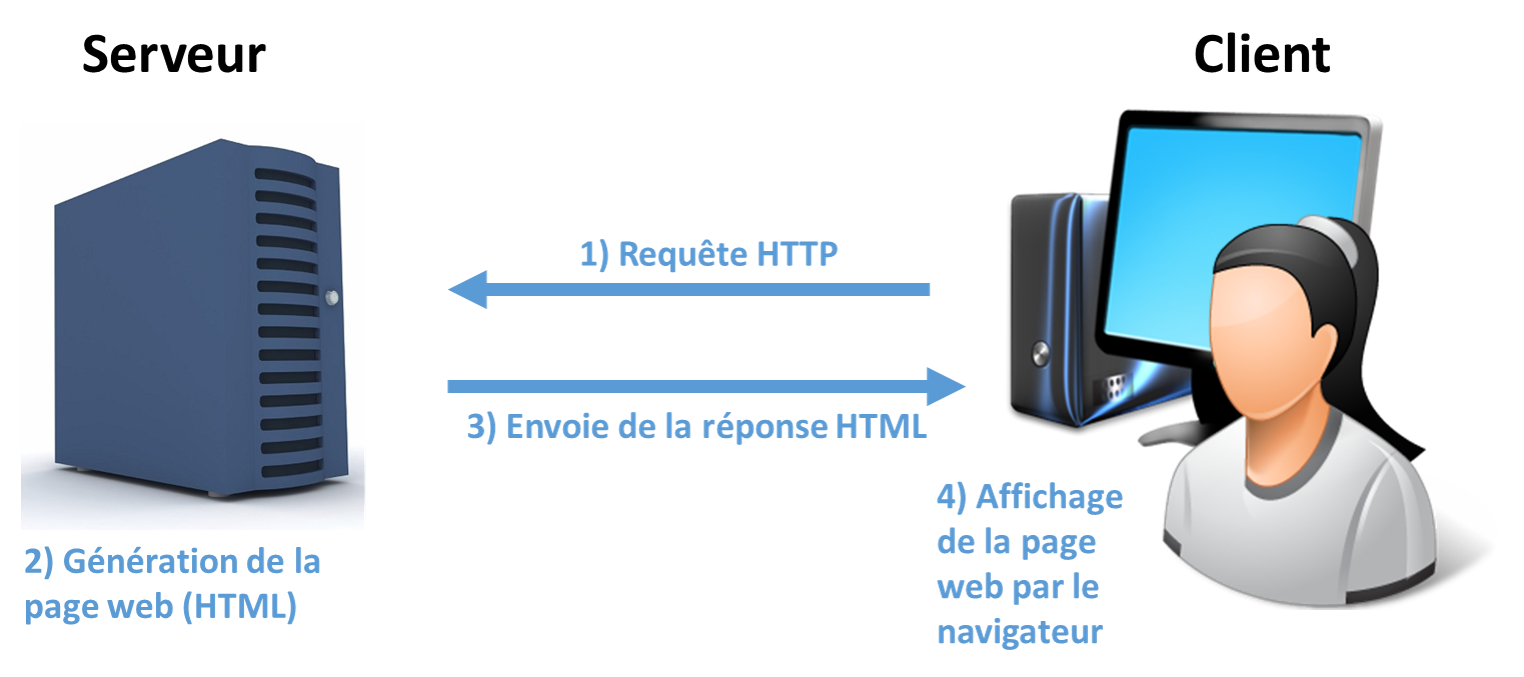
\includegraphics[width=10cm]{../img/part3/client_serveur.png}
				\caption{\label{modele_donnee} Le serveur génère dynamiquement la page
				HTML qui sera affichée sur le poste client.}
			\end{figure}
			
			% Le navigateur interprète le HTML et en affiche le contenu correspondant
			
			% Dans le même temps, le serveur envoi au client des scripts Javascript. Le
			% client est capable d'interpréter ces scripts. Ils permettent de faire des
			% interactions entre l'utilisateur et l'application sans faire d'appel au
			% serveur
			
			\paragraph{}% Modèle AJAX
			Une variante du modèle client-serveur existe, il s'agit du modèle AJAX. La
			limite du modèle précédent est que toute la page doit être renvoyée par le
			serveur a chaque requête (par exemple dès que l'utilisateur fait une action
			sur la page). Cela pose deux problèmes : d'une part beaucoup de données
			transitent entre le client et le serveur, d'autre part le rechargement
			complet de la page prend du temps ce qui nui à l'expérience de l'utilisateur.
			Le modèle AJAX, sur lequell repose TrackCIS, consiste à ne recharger que les
			parties de la page qui sont nécessaire sans toucher aux autres. Par exemple,
			dans le cas de l'affichage de la liste des messages entre une date de début
			et une date de fin, si l'utilisateur modifie la période, seule la liste des
			messages sera rechargée. Le reste de la page (menu, pieds de page,
			entête\ldots) ne changera pas.
			
		\subsection{TrackCIS est composé d'un frontal et d'une API}
			\paragraph{}% Archi générale de l'application
			TrackCIS est divisée en deux parties
			
			\begin{figure}[H]% Architecture globale de l'application
				\centering
				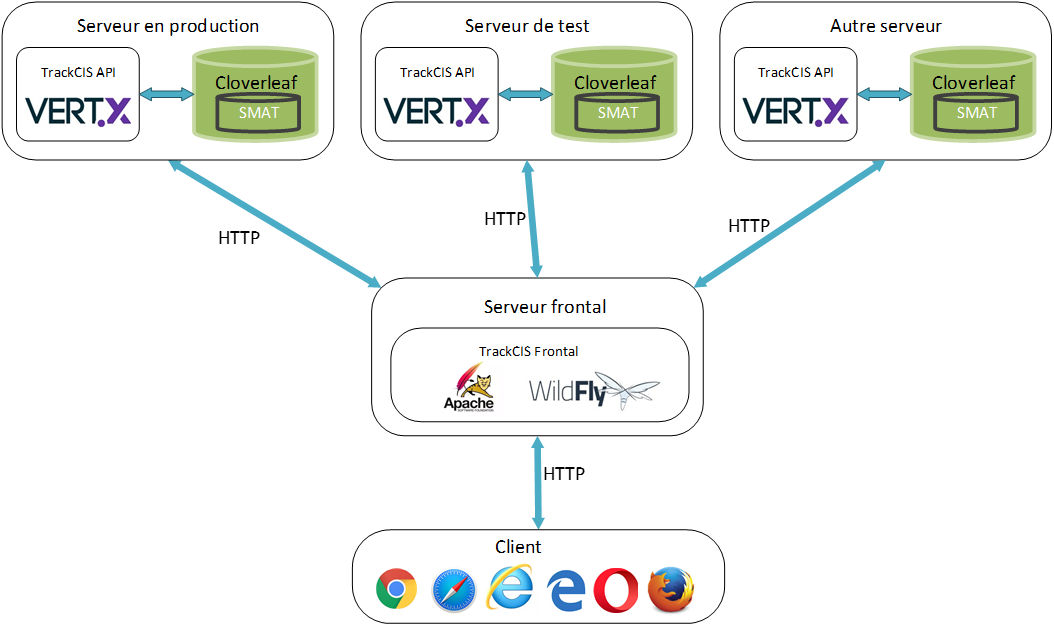
\includegraphics[width=10cm]{../img/part3/archi_trackcis.png}
				\caption{\label{archi_trackcis} TrackCIS est composés de deux éléments
				distincts pouvant se trouver sur des serveurs différents.}
			\end{figure}
			
			\paragraph{}% Les bases de java et de la POO
			Le frontal et l'API sont tous deux développés avec le langage Java.
			
		\subsection{Le frontal est développé en java J2EE}
			\paragraph{}% les grandes lignes de l'archi du front
			Java Entreprise Edition, que nous désignerons par J2EE, est une
			plateforme (un ensemble de bibliothèques) basée sur le langage Java et
			destinée au développement web.
			
		\subsection{L'API permet de communiquer avec Cloverleaf}
			\paragraph{}% Les grandes lignes de l'archi de l'API
			L'API est développée avec la plateforme standard de Java ou Java SE (Standard
			edition) qui n'est pas destinée au développement web.
	
	\section{L'analyse technique permet d'implémenter le nouveau module sur
	l'existant}
		\paragraph{}
		A présent que nous savons comment est construit TrackCIS, nous pouvons
		commencer la conception de la solution. Cette phase précède le développement à
		proprement parler. On cherche a définir tous les éléments techniques qui
		composerons le module statistique de TrackCIS, à savoir :
		\begin{itemize}
		  \item L'architecture, autrement dit la manière dont le code est structuré
		  \item Les outils utilisés, les bibliothèques, frameworks\ldots
		  \item Le modèle de données
		  \item 
		\end{itemize}
		
		\begin{figure}[H]% Méthodo de la conception
			\centering
			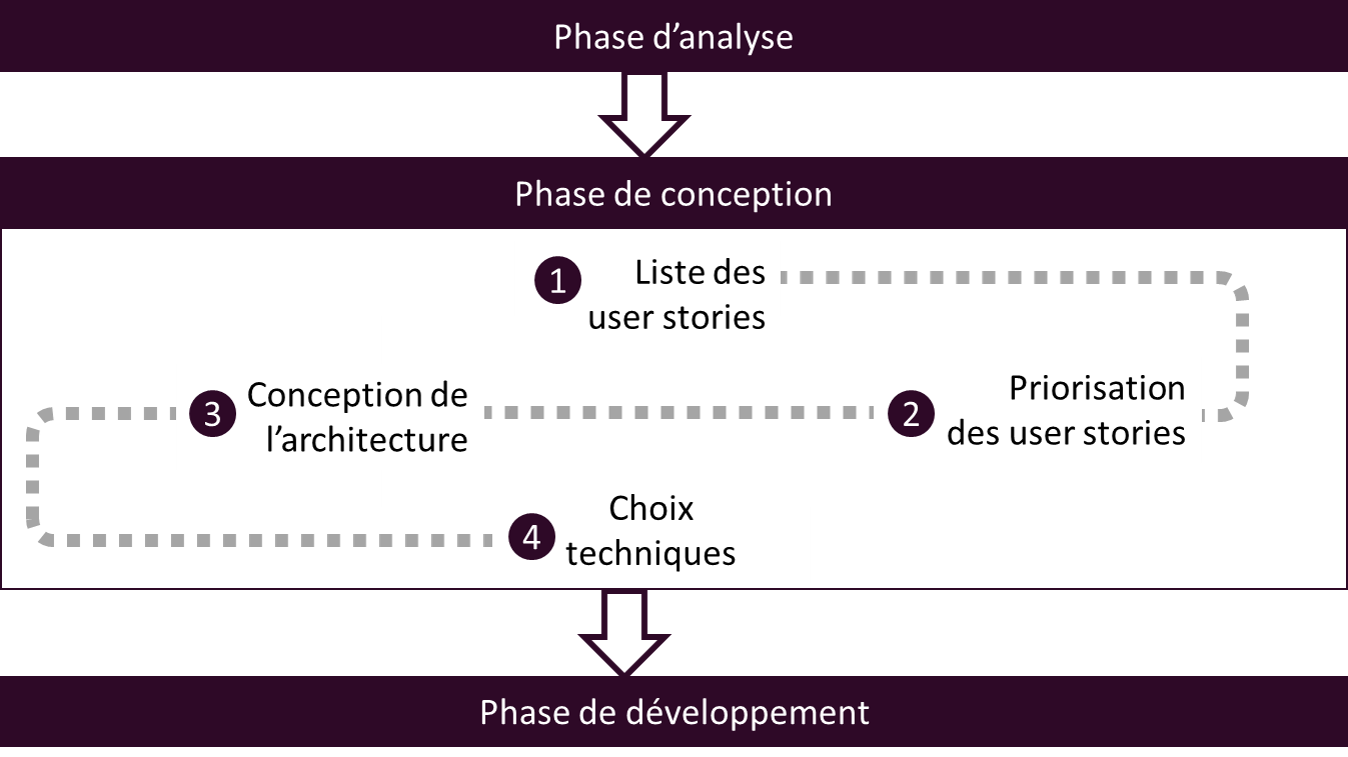
\includegraphics[width=15cm]{../img/part3/methodo_conception.png}
			\caption{\label{methodo_conception} Méthodologie de la conception du
			nouveau module.}
		\end{figure}
		
		\subsection{Un module qui est basé sur les données disponibles dans
		Cloverleaf}
		\subsection{Nouvelle architecture de l'application}
			\paragraph{}% Une archi dessinée à partir des contraintes fonctionnelles
			Le module statistique de TrackCIS doit~:
			\begin{itemize}% Liste des contraintes
			  \item être basé sur l'architectture déjà en place. Il n'est pas question
			  dans ce projet de faire de grosses modifications sur l'existant. Ceci est
			  valable aussi bien pour le code lui-même que pour la structure de la base
			  de donnée.
			  \item être fermé à la modification et ouvert à l'extention. C'est-à-dire
			  qu'il doit être possible, pour une équipe de développement ultérieur,
			  d'ajouter des fonctionnalités au module sans ajour à modifier le code
			  existant.
			  \item ne pas perturber le fonctionnement de Cloverleaf. Pour afficher des
			  données pertinentes pour l'utilisateur, certains traitements seront
			  nécessaires sur les données brutes. Ceux-ci peuvent cependant ralentir ou
			  perturber le fonctionnement de Cloverleaf. Il est nécessaire pour cela que
			  ces traitements ne soient pas fait sur le serveur de l'EAI, donc pas au
			  niveau de l'API.
			  \item ne pas surchager le serveur sur lequel est déployé le frontal. Le
			  serveur servant à héberger le frontal n'est pas forcément une machine très
			  puissante, bien que cela varie en fonction des établissements.
			\end{itemize}
			
			\begin{figure}[H]
				\centering
				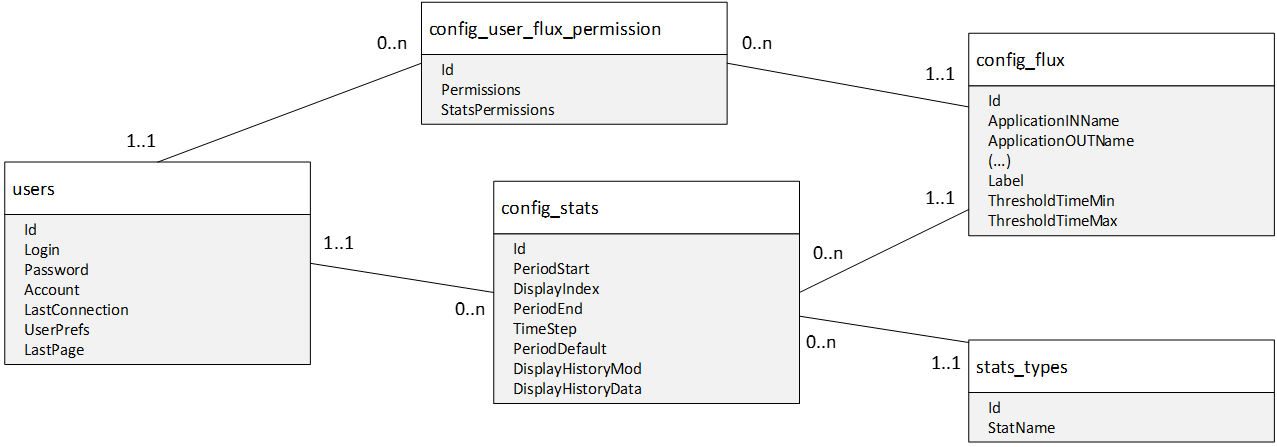
\includegraphics[width=16cm]{../img/part3/modele_donnee.png}
				\caption{\label{modele_donnee} Le nouveau modèle de donnée de TrackCIS au
				niveau du frontal.}
			\end{figure}
			
		\subsection{Réalisation des choix techniques}
			\paragraph{}% Liste des choix
			Le développement de ce projet implique l'utilisation d'un certain nombre de
			technologies. Certaines d'entre elles n'ont pas été utilisée pour le
			développement de la première version de TrackCIS.
			Le tableau ci-dessous résume l'ensemble des technologies qui ont été
			utilisées pour le développement de TrackCIS jusqu'a présent (c'est-à-dire
			avant le présent travail).
			
			\paragraph{}% Méthodo des choix
			Nous n'allons pas ici détaillé tous les choix techniques qui ont été fait.
			Nous mettrons en avant dans cette partie la méthodologie avec laquelle ces
			différents choix tecnique on été effectué en l'illustrant d'un exemple, en
			l'occurence le choix de la bibliothèque graphique javascript. Comme nous
			l'avons vu dans l'architecture de nouveau module, les graphiques sont
			dessinés par le navigateur client. La navigateur reçois un ensemble de script
			javascript qu'il sait interpréter. Certains de ces scripts permettrons donc
			d'afficher les graphiques. Pour cela nous avons besoin d'une bibliothèque
			javascript, c'est-à-dire un ensemble de fonctions précrites. Il en existe de
			très nombreuses et certaines sont gratuites et libres. Pour faire notre choix
			nous partons des contraintes suivantes~:
			\begin{itemize}
			  \item La bibliothèque doit être gratuite et son utilisation pour la
			  création de produits commerciaux doit l'être également.
			  \item Elle doit permettre à minima de dessiner les types de graphiques
			  spécifiés dans les fonctionnalités (courbe et historgamme avec plusieurs
			  séries de données, jauge et donut).
			\end{itemize}
			% Listing des librairies qui répondent à ces critères
			Nous retenons une liste de N bibliothèques qui respectent ces deux critères.
			Pour n'en retenir qu'une nous les comparons à l'aides d'autres critères qui
			sont~:
			\begin{itemize}
			  \item La qualité et la disponibilité de la documentation et de la
			  communauté d'utilisateur. Il est importatn de penser à la suite du projet
			  et aux améliorations future du module. Une bonne documentation nous
			  permettra d'aller plus vite dans l'implémentation et également à une équipe
			  de développement ultérieur de s'approprier plus facilement le code pour y
			  ajouter des graphique ou corriger des bugs.
			  \item L'estétisme et la possibilité de personalier les graphique. Certaines
			  bibliothèque propose des graphiques prêts à l'emplois, ce qui présente un
			  gain de temps certain pour le développement. Cependant, le module
			  statistique doit respecter la charte graphique déjà en place dans l'outil.
			  \item La possibilité de faire de petites animations de transition. Cela
			  peut être par exemple un petit effet à l'appartion d'une courbe, ou la
			  possibilité d'afficher une infobulle lors du passage de la sourie sur un
			  point de donnée du graphique.
			  \item La possibilité de pouvoir dessiner d'autres types de graphique. Nous
			  ne pouvons pas prévoir comment évolura le module ni quelles nouvelles
			  données seront rendu accessibles par Cloverleaf dans le future. Nous devons
			  choisir une bibliothèque nous laissant suffisament de possibilité pour
			  pouvoir représenter d'autres types de graphiques.
			\end{itemize}
			Tous ces critères ne sont pas égaux, certain sont plus important que
			d'autres. C'est pourquoi nous allons les pondérer à l'aide d'une note sur
			dix. Nous notons ensuite les six bibliothèques retenue sur chacun de ces
			critère, puis nous appliquons la pondération à chaque note. La note globale
			de chaque bibliothèque est le total des notes podérées de chque critère. Le
			tableau \ref{choix_bib_js} présente le résultat de cette méthode.
			\begin{table}[H]
				\centering
				\caption{\label{choix_bib_js} Choix de la bibliothèque graphique
				javascript : d3js se démarque des autres.}
				\begin{tabular}{| p{2cm} | p{2cm} | p{2cm} | p{2cm} | p{2cm} |
				p{2cm} | p{2cm} |}
					\hline
						\thead{Bibliothèque}
						&\thead{Documentation}
						&\thead{Simplicité d'utilisation}
						&\thead{Esthétisme}
						&\thead{Annimations}
						&\thead{Autres graphiques possibles}
						&\thead{Total}
						\\
					\hline
						D3&10&1&10&10&10&\thead{244}
						\\
					\hline
						Google Charts&10&9&5&5&9&\thead{230}
						\\
					\hline
						Chartist&8&6&8&10&5&\thead{202}
						\\
					\hline
						EJS Chart&7&8&7&2&8&\thead{196}
						\\
					\hline
						JQPlot&6&8&6&5&8&\thead{186}
						\\
					\hline
						RGraph&6&9&2&4&5&\thead{146}
						\\
					\hline
				\end{tabular}
			\end{table}
			La bibliothèque retenue est D3 (Data driven document), 
			open source et gratuite permettant de construire n'importe quel type de
			visualisation de données.
			
	\section{Une gestion de projet en mode agile}
		\paragraph{}
		La phase de conception est maintenant terminée et les choix technique
		réalisés. Nous pouvons à présent passer à l'implémentation à proprement
		parler, c'est à dire à la production du code.
		
		\subsection{Une méthodologie qui s'inspire des méthodes agiles}
			\paragraph{}% C'est quoi l'agilité et pourquoi ce choix
			
			L'<<équipe>> projet étant composée d'une seule personne, moi, je vais bien
			niquer ma race !
			
			\paragraph{}% Les sprints
			
			\paragraph{}% Le backlog et les US
			
			
			
			\begin{figure}[H]% Méthodo du développement
				\centering
				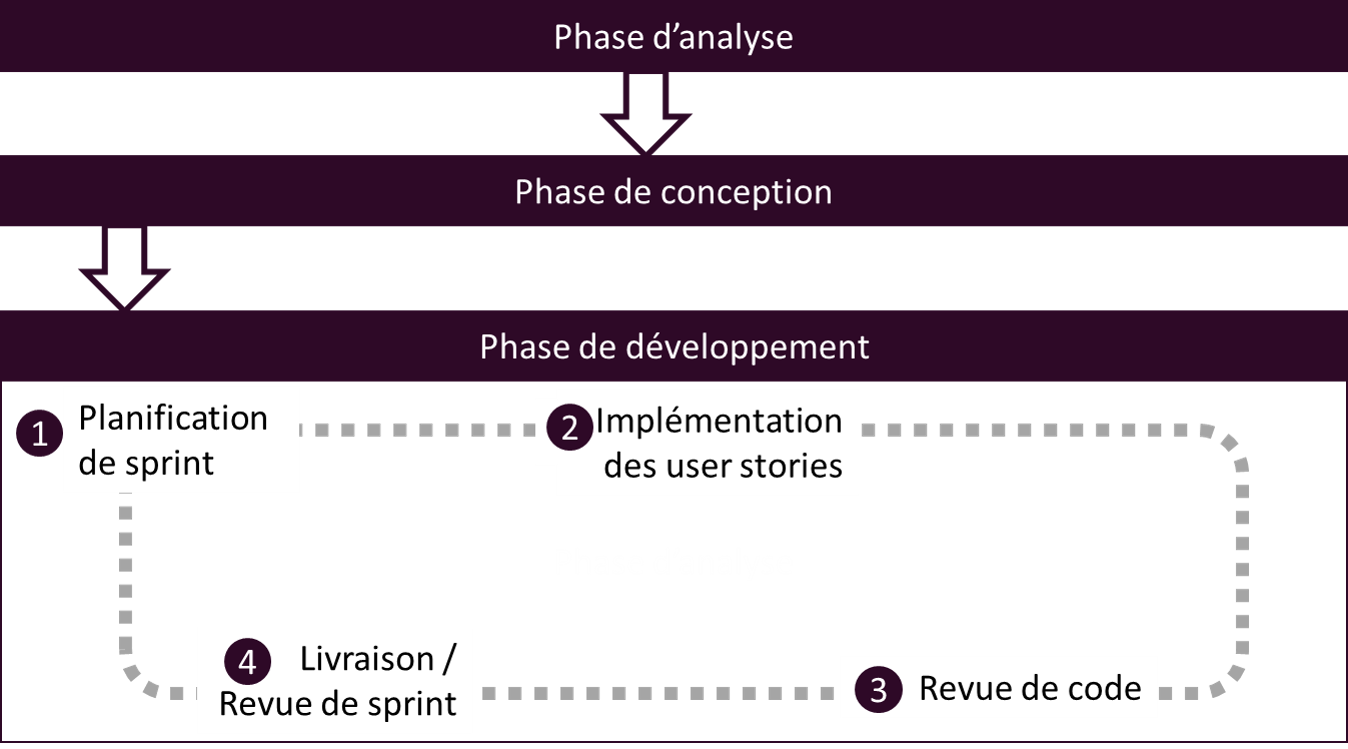
\includegraphics[width=15cm]{../img/part3/methodo_dev.png}
				\caption{\label{methodo_dev} Le développement se déroule en sprints de
				deux semaines chacun.}
			\end{figure}
		
		\subsection{Élaboration du backlog}
			\paragraph{}% Passage des fonctionnalités aux user stories
			
			
			Pour construire notre backlog, nous devont établir une liste de user sotries.
			De la même manière que nous avons établi un lien entre besoins et
			fonctionnalités, il est possible de relier ces dernières aux user stories.
			Une fonctionnalité peut être découpée en plusieurs user stories, comme le
			montre la figure \ref{mapping_fonctios_us}, une user story n'est liée qu'à
			une seule fonctionnalité.
			\begin{figure}[H]% Mapping fonctionnalités -> US
				\centering
				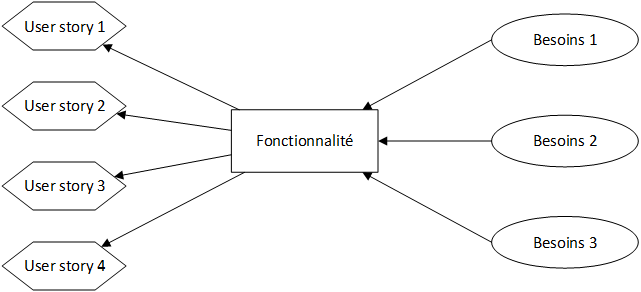
\includegraphics[width=7cm]{../img/part3/mapping_fonctios_us.png}
				\caption{\label{mapping_fonctios_us} Chaque fonctionnalité est redécoupée
				en une ou plusieurs user stories.}
			\end{figure}
			
			\paragraph{}% Priorisations des US
			Le backlog est la base de travail pour le développement. C'est à la fois
			unoutil de spécification décrivant finement les fonctionnalités du module, et
			un outil de gestion de projet car il permet de suivre son avancement. Le
			backlog permet également de planifier le travail. Pour cela il faut en
			prioriser les élements.\newline
			
			
			Pour estimer la difficulté intrinsèque au développement de chaque user story,
			nous emploirons la technique dite du planing poker. Nous utiliserons comme
			base les premiers éléments de la suite de Fibonacci (1, 2, 3, 5, 8, 13, 21,
			34,\ldots). Nous attriburons une note médianne à une storie que nous
			évaluerons de difficulté moyenne. En l'occurence % TODO
			
			Puis nous noterons les autres stories à relativement à la première en
			n'utilisant que des éléments de la suite de Fibonacci.
			
	
	\section{Bilan de la phase de développement et suite du projet}
		\paragraph{}
		Cette dernière partie est l'occasion de faire le bilan sur ce qui a été
		implémenté.
		
		\subsection{Les fonctionnalités implémentées}
			\paragraph{}% Bilan quantitatif de ce qui a été fait et reste à faire
		
			\paragraph{Historique de nombre de messages par flux~: }
			
			\paragraph{Valeur moyenne du temps de transfert d'un message dans le flux~: }
		
		\subsection{Les limites du projet}
			\paragraph{}% présentation
			Tout au long de ce prjet nous avons été amené à faire un certain nombre de
			choix, parfois de manière très arbitraire. Revenous ici sur les principales
			limites de la méthodologie globale du projet visant à améliorer TrackCIS et
			voyons comment nous pouvons en tirer les leçons pour préparer la suite du
			projet.
		
			\paragraph{}% Le choix de développer le module statistique est arbitraire
			
			\paragraph{}% La priorisation (besoins, fonctios et US) sont aussi
			% arbitraires
			
		\subsection{Les suites possibles du projet pour Xperis}
			\paragraph{}% Les gros modules a développer à partir de l'ADB
			
			\paragraph{}% Les <<petites>> amélioration à faires
			
			